\section{Missing transverse energy}
\label{chp:obj:met}

The ATLAS subdetectors are not sensitive to neutral weakly-interacting particles like neutrinos or particles predicted in BSM scenarios (e.g. WIMPs, neutralinos). Those particles pass through the ATLAS detector without leaving any electric signals, thus creating an apparent imbalance of
the total measured momentum in the transverse plane.\par The missing transverse momentum, $\vec{p}_{\rm T}^{\rm miss}$, is obtained from the negative vector sum of the $\pt$ of all particles detected in a $pp$ collision. The magnitude and the direction of this vector are respectively the missing transverse energy, \MET, and the missing energy azimuthal angle, $\phi^{\rm miss}$.
The \MET reconstruction \cite{ATL-PHYS-PUB-2015-023} is characterised by two contributions: the hard term from all reconstructed objects (electrons, muons, photons, $\tau$-leptons and jets) and the soft term consisting of reconstructed charged particle tracks not associated with the hard physics objects. To avoid a double-counting of contributions,  physics objects are considered in a specific order: electrons, photons, then hadronically decaying $\tau$-leptons, muons and finally jets. The lower priority particle-like objects ($\gamma$, $\tau$) are fully rejected if they share their calorimeter signal with an electron that has already entered the \MET reconstruction. Jets can still partially contribute to \MET, if not more than $50\%$ of their signal is already used by an overlapping particle with higher priority.
After all \MET contributions from hard objects are collected, ID tracks from the hard-scatter PV, but not associated with any of the accepted contributing hard objects, are used to construct the soft term.
The reconstruction of \MET should be consistent with the final state selected in a given analysis. Rejecting certain electrons, if the corresponding calorimeter signal is collected with the new assumption, can change the \MET.
The flexibility needed to re-calculate \MET under changing analysis requirements for the same event is implemented using dedicated variables corresponding to a specific object contribution. In this approach, the full $\vec{p}_{\rm T}^{\rm miss}$ is the vectorial sum of missing transverse momentum terms:

\be
\vec{p}_{\rm T}^{\,\rm miss}= \underbrace{- \displaystyle\sum_{\substack {\text{electrons}}} \vec{p}_{\rm T}^{\,e} - \displaystyle\sum_{\substack {\text{photons}}} \vec{p}_{\rm T}^{\,\gamma} - \displaystyle\sum_{\substack {\text{$\tau$-leptons}}} \vec{p}_{\rm T}^{\,\tau} - \displaystyle\sum_{\substack {\text{muons}}} \vec{p}_{\rm T}^{\,\mu}- \displaystyle\sum_{\substack {\text{ jets}}} \vec{p}_{\rm T}^{\,\rm jet} }_{\text{hard term}}\underbrace{-\displaystyle\sum_{\substack {\text{unused}\\ \text{tracks}}} \vec{p}_{\rm T}^{\,\rm track}}_{\text{soft term}}
\label{eq:obj:met:metdef}
\ee

The sum over electron and muons runs over the selected ones because electrons enter in the calculation first and muons rarely have a calorimetric deposit that overlaps with other objects. The hard term has a little dependence on pileup as the objects used already include pileup corrections. The particular choice of using only tracks from the hard-scatter PV for the soft term strongly suppresses pileup contributions to this term as well.\\

The performance of \MET reconstruction is evaluated in several topologies:
\bi
\ib $Z\to \ell^{+}\ell^{-}$ events are an ideal final state for the evaluation of \MET reconstruction performance (possible both in data and MC) since the events have no intrinsic missing transverse momentum. Scale and resolution measurements in this final state will be indicative of detector limitations affecting the reconstruction quality.
\ib $W\to \ell \nu$ events provide a good benchmark sample with intrinsic \MET arising from the non-zero neutrino $\pt$. In this sample it is possible (only in MC) to validate scale, resolution and direction of the reconstructed \MET.
\ib $t\bar{t}$ events allow measurements of \MET performance in events with multiple energetic jets in the final state (possible in both data and MC).
\ei

Deviation of the observed \MET from the expectation is used to measure the \MET response. If this deviation is independent of the genuine missing transverse momentum, or any other hard $\pt$ indicative for the overall hard scatter activity, the \MET response is linear. Detector inefficiencies and limited detector coverage limitation introduce a bias and are expected to translate into a non-linear response. The \MET response and resolution in $W\to \ell \nu$ and $t\bar{t}$ events is shown in figure \ref{fig:obj:met:resoresp}.

\begin{figure}[h!]
\begin{subfigure}{0.5\textwidth}
  \centering
  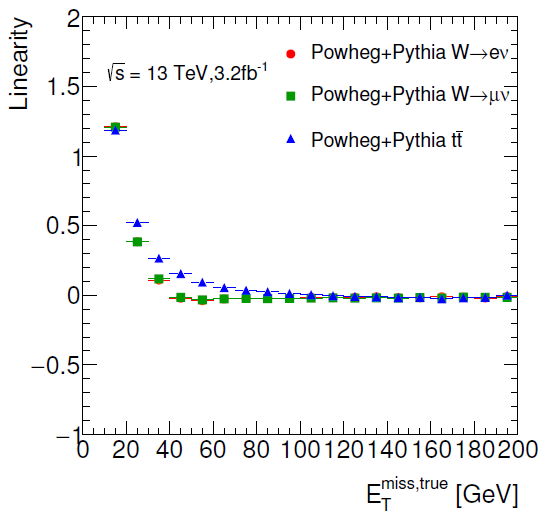
\includegraphics[width=0.9\textwidth]{figures/Objects/metresponse.png}
  \caption{}
  \label{fig:obj:met:resolution}
\end{subfigure}
\begin{subfigure}{0.5\textwidth}
  \centering
  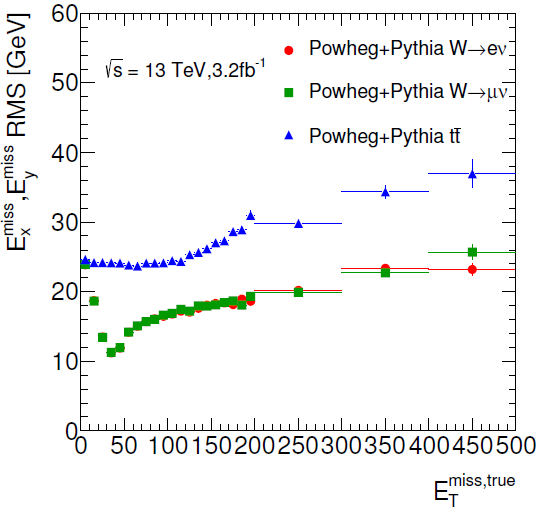
\includegraphics[width=0.9\textwidth]{figures/Objects/metresolution.png}
  \caption{}
  \label{fig:obj:met:response}
\end{subfigure}
\captionsetup{width=0.85\textwidth} \caption{\small The \MET (a) response and (b) resolution evaluated in $W\to \ell \nu$ and $t\bar{t}$ simulated events. From reference \cite{ATL-PHYS-PUB-2015-023}.}
\label{fig:obj:met:resoresp}
\end{figure}


Systematic uncertainties affecting the \MET computation depend on the composition of the hard term and the magnitude of the resulting soft term. For the former, systematic uncertainties on the physics object calibrations are directly translated into the \MET computation through equation \ref{eq:obj:met:metdef}. Systematics uncertainties affecting the soft term are evaluated in $Z\to e^{+}e^{-}$ events. Uncertainties of $\sim10\%$ and $\sim20\%$ have been assigned to the resolution and scale respectively.



